\documentclass[12pt]{exam}
\usepackage[phy]{template-for-exam}
\usepackage{circuitikz,ifthen,multicol,siunitx}
\usepackage[margin=0.5in]{geometry}
\footer{}{}{}
\header{}{}{}
\shadedsolutions
\printanswers
\usetikzlibrary{shadings,decorations.pathmorphing,arrows.meta,patterns}

\def\mystrut{\protect\rule[-2.2ex]{0ex}{2.2ex}} 
\qformat{ \textbf{Task \#\thequestion}
  \ifthenelse{\equal{\thequestion}{\thequestiontitle}}
    {}
    {: \emph{\thequestiontitle}}
  \mystrut  \hfill}

\begin{document}




\begin{questions}


\question
  Find the current going through the battery in each of the circuits below:

  \begin{parts}
    \part \hfill

      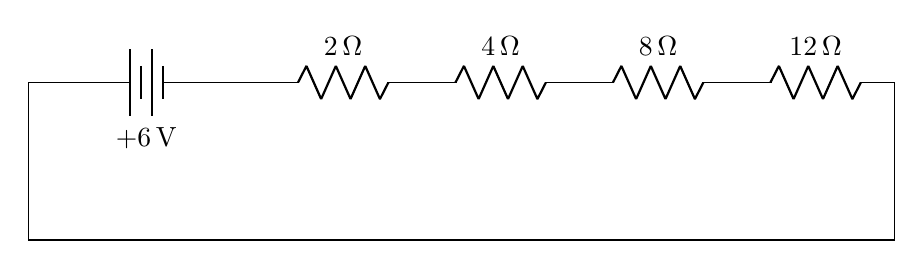
\begin{tikzpicture}
        \draw (0,0) 
          to                               ++(0,2)
          to[battery,l_=$+\SI{ 6}{\volt}$] ++(3,0)
          \foreach \x in {2,4,8,12}{
            to[R=\SI{\x}{\ohm}]            ++(2,0)
          }
          |- (0,0);
      \end{tikzpicture}
    
    \part \hfill
    
      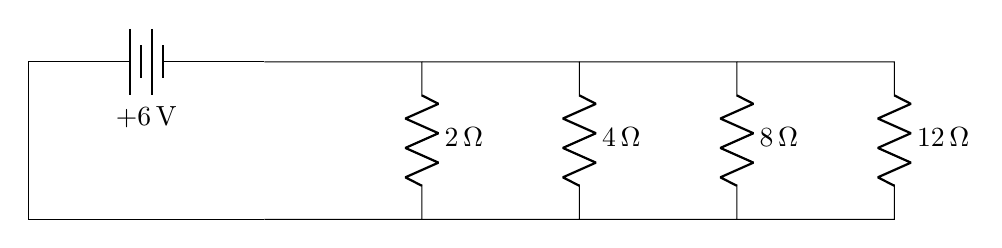
\begin{tikzpicture}
        \draw (0,0) 
          to                               ++(0,2)
          to[battery,l_=$+\SI{ 6}{\volt}$] ++(3,0)
            coordinate (a);
        \draw (a) ++(0,-2) -- (0,0);
        \foreach \x in {2,4,8,12}{
          \draw (a) -- ++(2,0) coordinate (a)
            to[R=\SI{\x}{\ohm}] ++(0,-2) 
            to                  ++(-2,0);
        }
      \end{tikzpicture}
   
  \end{parts}


\vs \hrule \vs

\question
  Find the current going through the battery in the circuit below.
    
    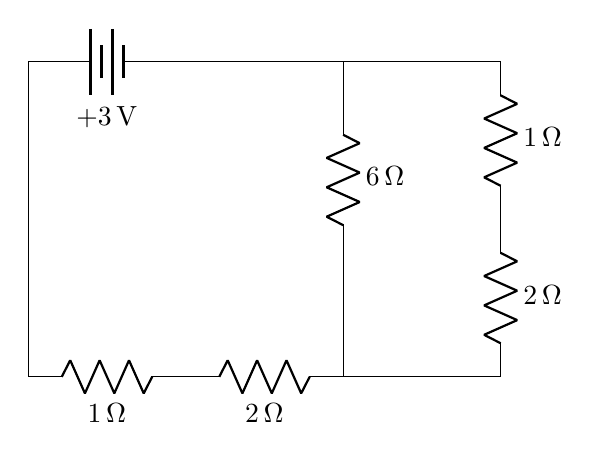
\begin{tikzpicture}
      \draw (0,0) 
        to                     ++(0,4)
        to[battery,l_=$+\SI{ 3}{\volt}$] ++(2,0)
        to                     ++(2,0) coordinate (a)
        to[R,l=\SI{  6}{\ohm}] ++(0,-3)
        to                     ++(0,-1) coordinate (b)
        to[R,l=\SI{  2}{\ohm}] ++(-2,0)
        to[R,l=\SI{  1}{\ohm}] ++(-2,0);
      \draw (a)
        to                     ++(2,0)
        to[R,l=\SI{  1}{\ohm}] ++(0,-2)
        to[R,l=\SI{  2}{\ohm}] ++(0,-2)
        to (b);
    \end{tikzpicture}

\vs \hrule \vs


\question
  Find the current going through the battery in the circuit below.
    
    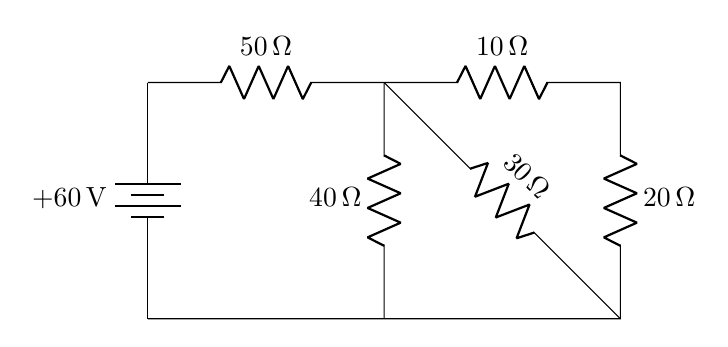
\begin{tikzpicture}
      \draw (0,3) 
        to[R=\SI{50}{\ohm}]              ++(3, 0) coordinate (a)
        to[R=\SI{10}{\ohm}]              ++(3, 0)
        to[R=\SI{20}{\ohm}]              ++(0,-3) coordinate (b)
        to                                 (0, 0);
      \draw (a) to[R,l_=\SI{40}{\ohm}]   ++(0,-3);
      \draw (a) to[R=\SI{30}{\ohm}]        (b);
      \draw (0,3) to[battery,l_=$+\SI{60}{\volt}$] (0,0);
    \end{tikzpicture}

    \vspace*{\stretch{1}}
  
\end{questions}








\end{document}